\documentclass[aspectratio=169]{beamer}

\usepackage{tikzlings}

\setbeamertemplate{navigation symbols}{}

% trick taken from https://topanswers.xyz/tex?q=1989
\tikzset{
    use page relative coordinates/.style={
        shift={(current page.south west)},
        x={(current page.south east)},
        y={(current page.north west)}
    },
}

\makeatletter
\newcommand*{\slideinframe}{\number\beamer@slideinframe}
\makeatother

\begin{document}

\def\steps{700}
\begin{frame}
  \begin{tikzpicture}[
      remember picture,
      overlay,
      use page relative coordinates,
    ]
  
    \node[anchor=north,inner sep=0pt] at (current page.north) {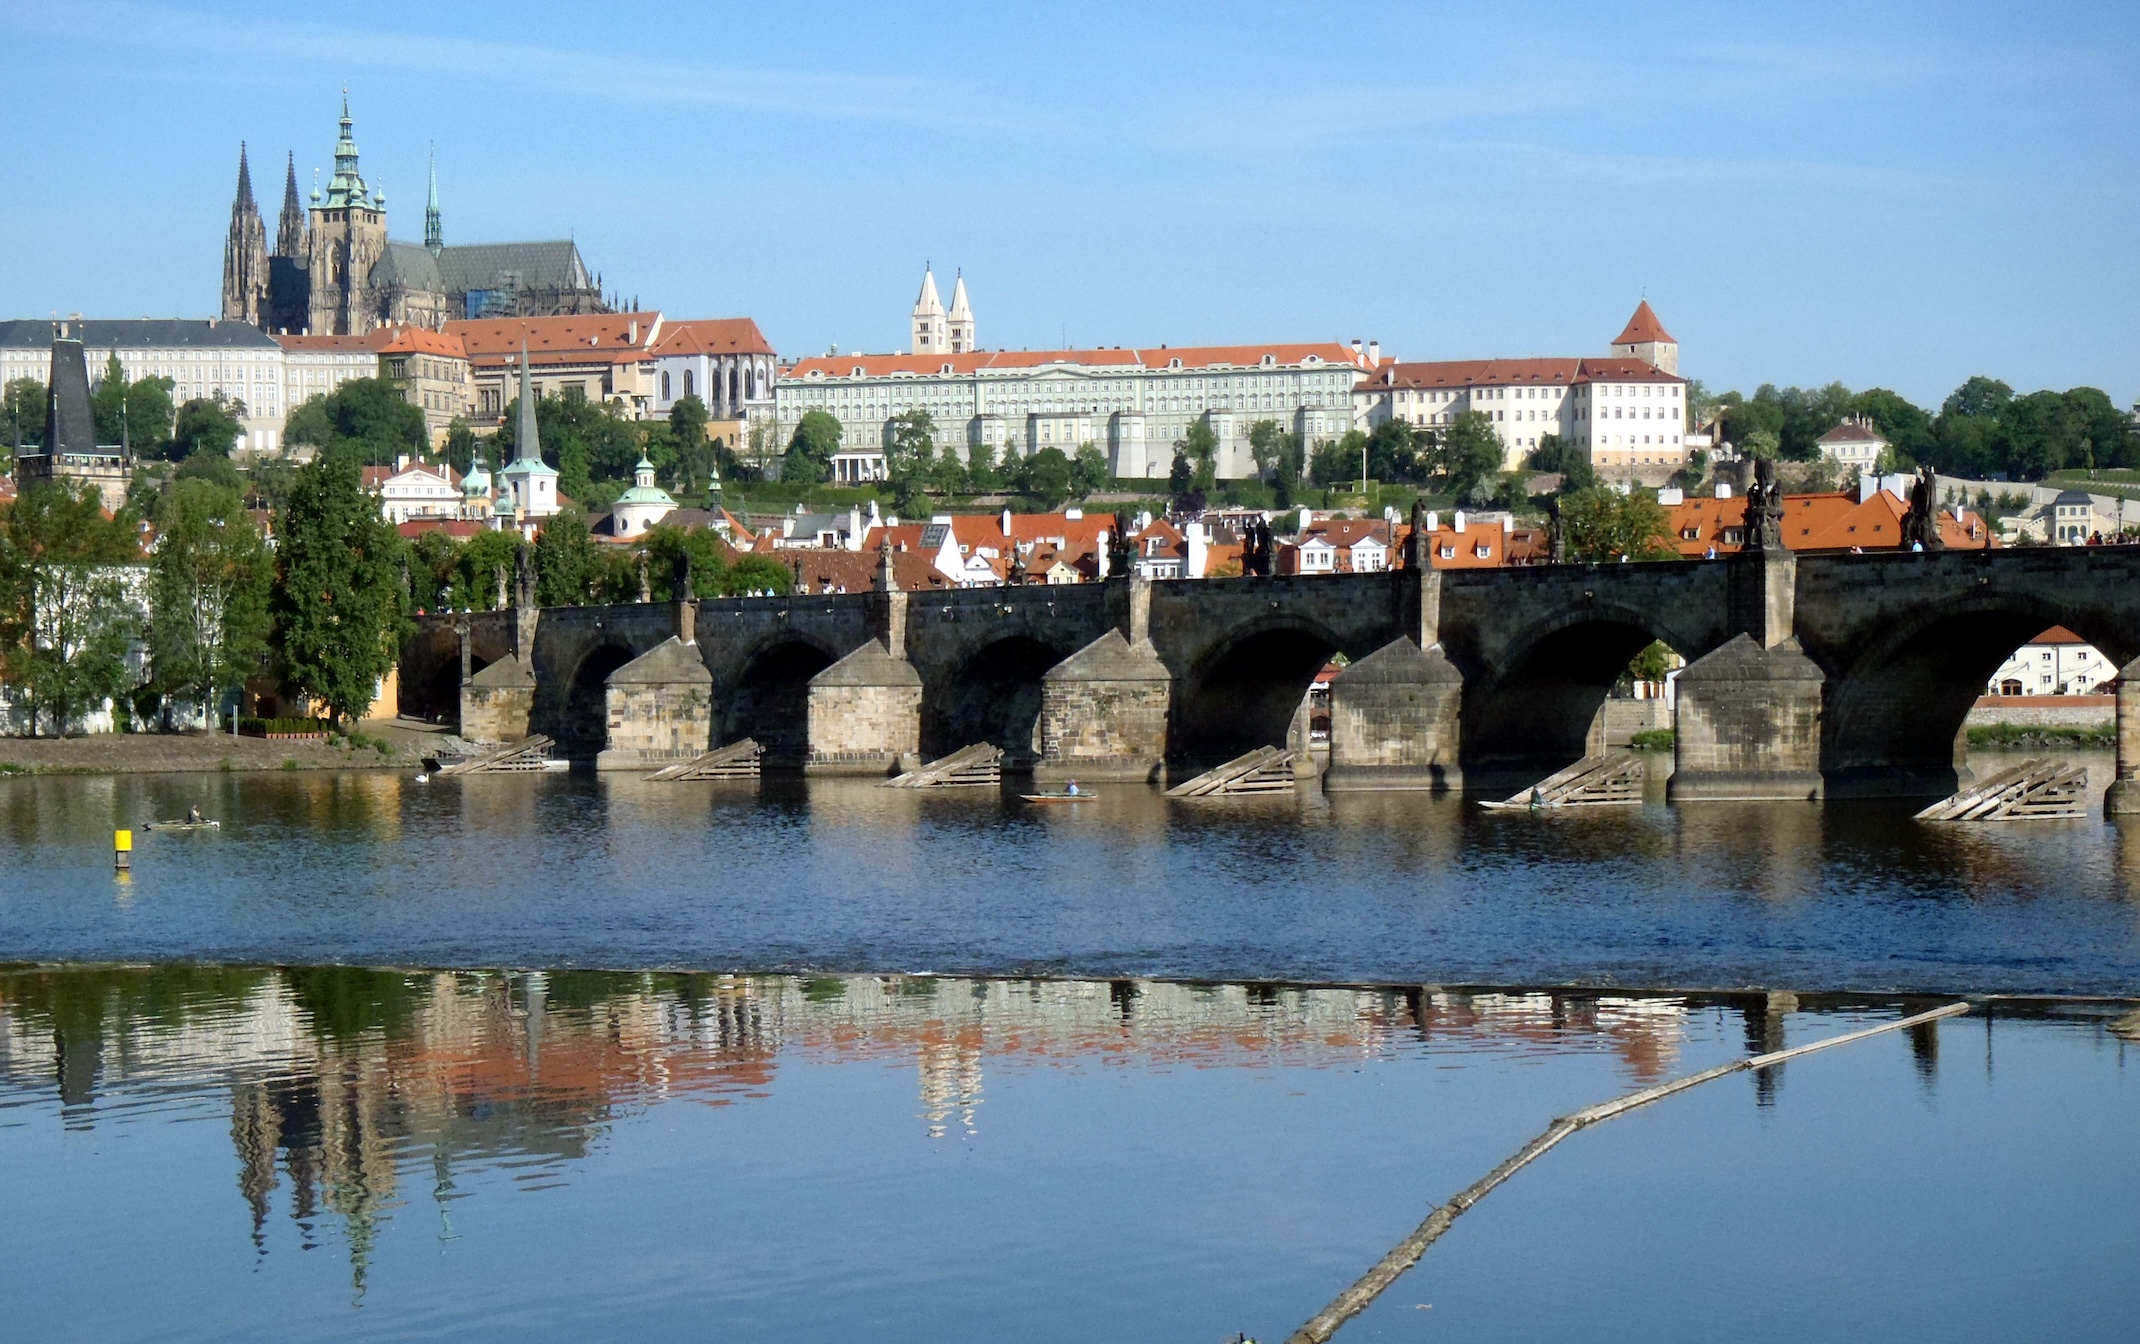
\includegraphics[width=\paperwidth]{Charles_bridge_and_Prazsky_Hrad_-_panoramio}};
    
    \node at (-0.5+1.5*\slideinframe/\steps,0.15+0.29*\slideinframe/\steps) {
\includegraphics[height=1cm]{clip_duck}};
    
    \node[anchor=north,inner sep=0pt] at (current page.north) {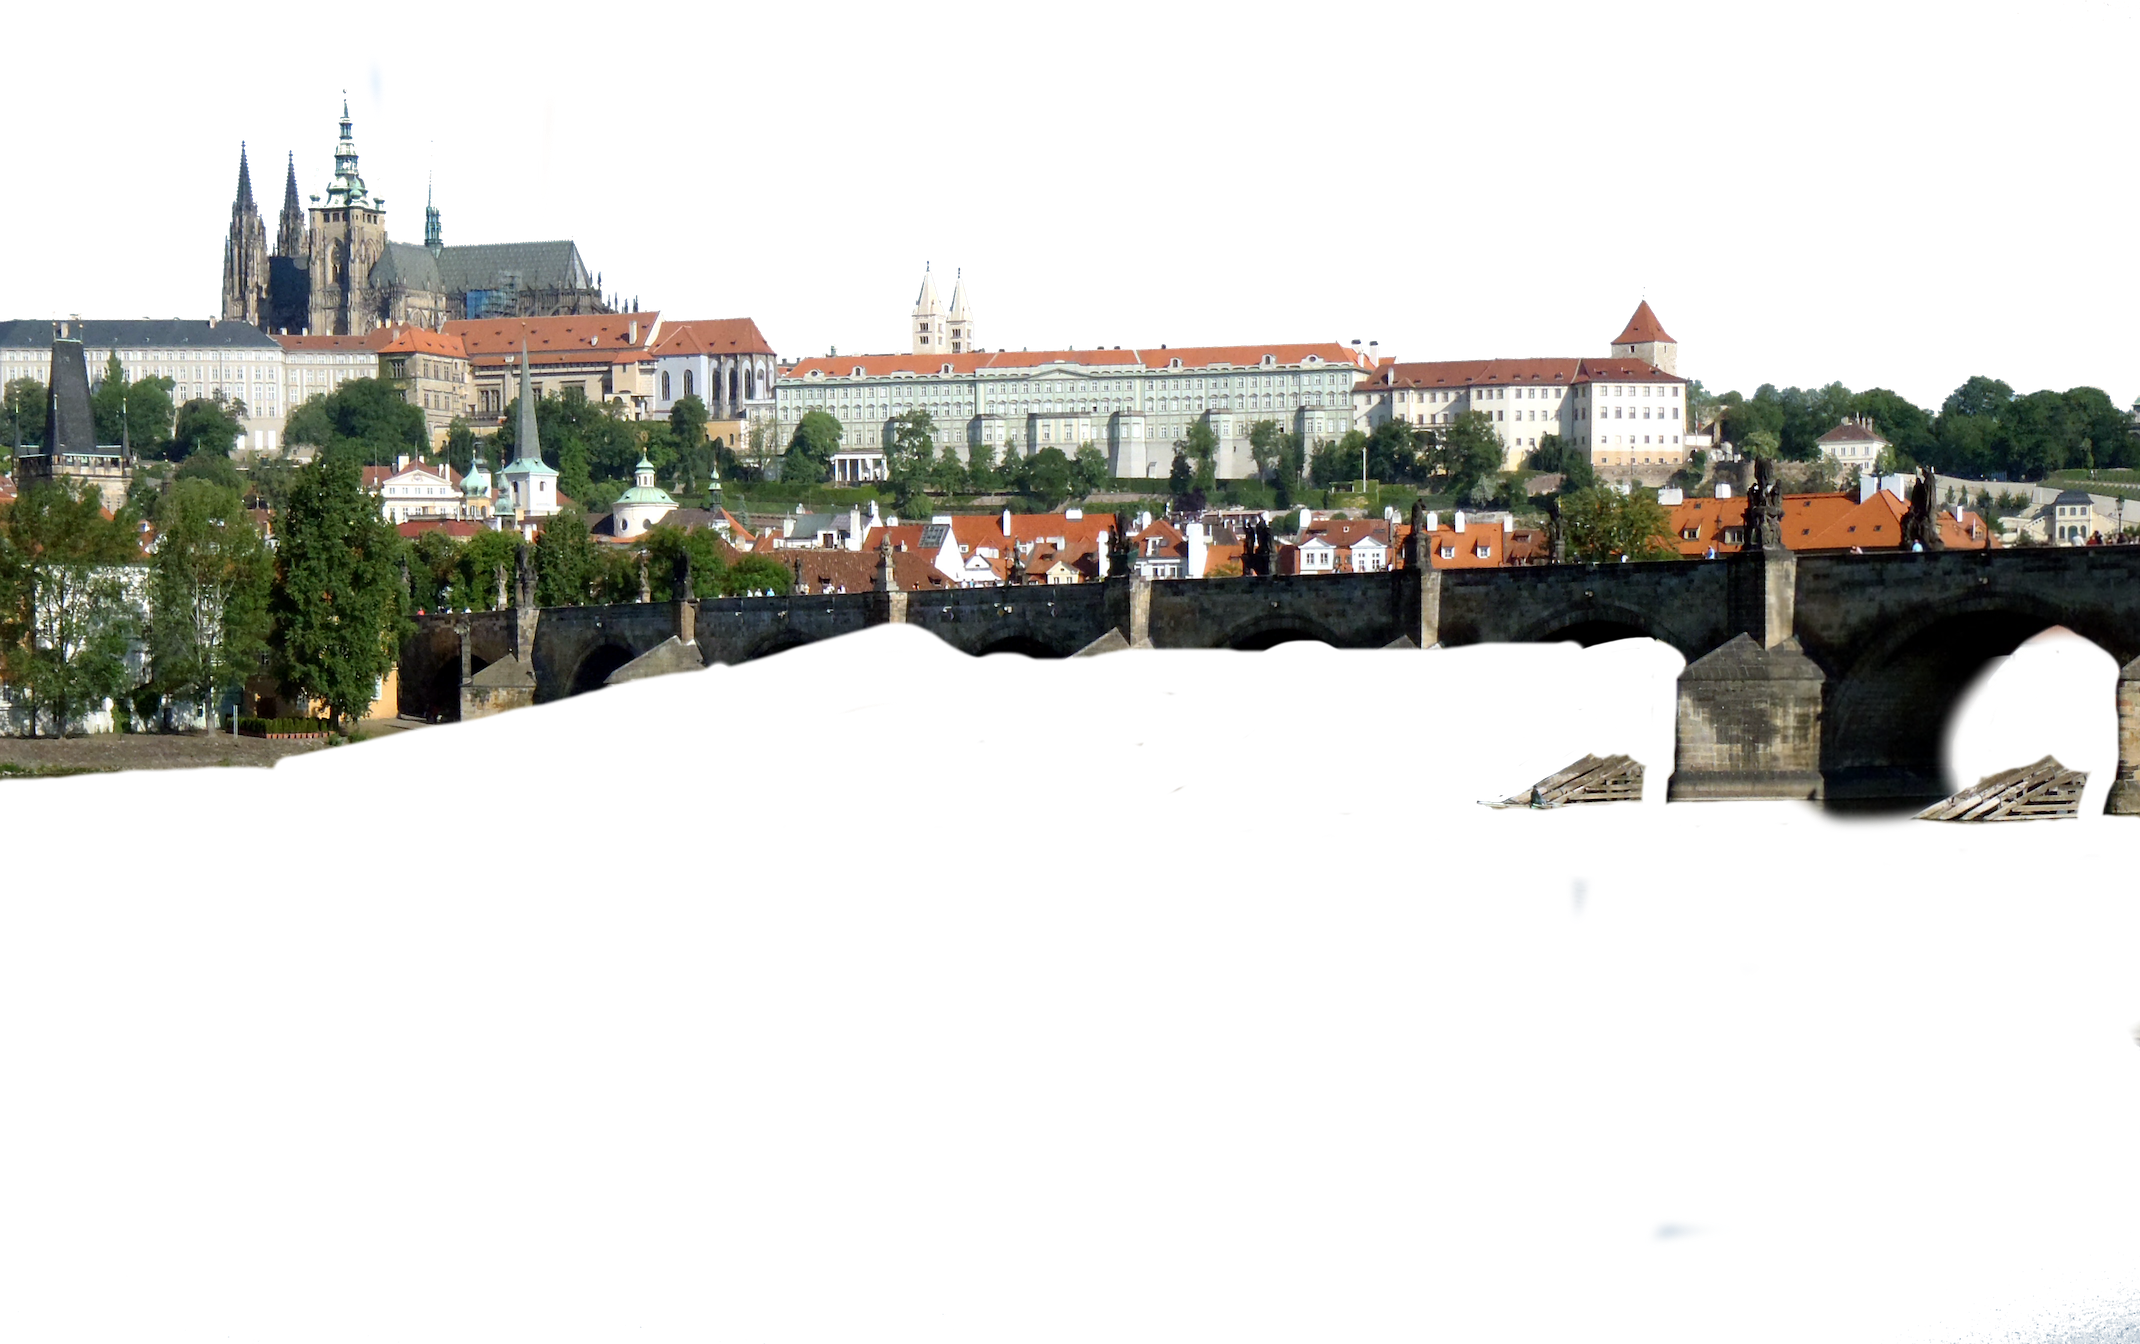
\includegraphics[width=\paperwidth]{Charles_bridge_and_Prazsky_Hrad_-_panoramio_fg}};
   
    \node at (-1.5+2*\slideinframe/\steps,-0.5+0.83*\slideinframe/\steps) {
\includegraphics[height=1cm]{clip_duck}};            
    
    \node at (-0.1+2*\slideinframe/\steps,-0.1+0.83*\slideinframe/\steps) {
\includegraphics[height=1cm]{clip_duck}};        

    % credit for background image
    \node[white,text width=\paperwidth,font=\tiny,align=center] at ([yshift=0.25cm]current page.south) {Image by Eric Spenle (\url{https://commons.wikimedia.org/wiki/File:Charles_bridge_and_Prazsky_Hrad_-_panoramio.jpg})};
    
  \end{tikzpicture}
  \pause[\steps]
\end{frame}

\end{document}